%%%%%%%%%%%%%%%%%%%%%%%%%%%%%%%%%%%%%%%%%%%%%%%%%%%%%%%%%%%%%%
%%%                                                        %%%
%%%   IMPORTANT - DO NOT ADD REVIEW QUESTIONS HERE         %%%
%%%                                                        %%%
%%%   REVIEW QUESTIONS MUST FIRST GO TO SOLUTION MANUAL,   %%%
%%%   THEN STRIPPED OFF SOLUTIONS AND GO HERE              %%%
%%%                                                        %%%
%%%%%%%%%%%%%%%%%%%%%%%%%%%%%%%%%%%%%%%%%%%%%%%%%%%%%%%%%%%%%%

\section{Introduction}

For all review questions in this book: None, one, or multiple
choices may be correct.

\begin{enumerate}
\item Name the university where Karel the Robot was created.
\begin{enumerate}
\item[A1] MIT
\item[A2] Princeton
\item[A3] Harvard
\item[A4] Stanford
\end{enumerate}
\item What is the programming language that you should learn after Karel?
\begin{enumerate}
\item[A1] C
\item[A2] Python
\item[A3] Haskell
\item[A4] Fortran
\end{enumerate}
\item What is the largest conceptual difference between Karel and standard
      procedural programming languages such as Python, C, C++ or Fortran?
\begin{enumerate}
\item[A1] Karel knows only five commands.
\item[A2] Karel can only do simple algorithms.
\item[A3] Karel does not know math.
\item[A4] Karel has only five sensors.
\end{enumerate}
\item Where does Karel live and what objects does he like to collect?
\begin{enumerate}
\item[A1] Karel lives in a maze and he likes to collect gems.
\item[A2] Karel lives in a cave and he likes to collect gold nuggets.
\item[A3] Karel lives on an island and he likes to collect coconuts.
\item[A4] Karel lives in a marketplace and he likes to collect coins from the ground.
\end{enumerate}
\item What is the command that moves the robot one step forward?
\begin{enumerate}
\item[A1] step
\item[A2] forward
\item[A3] go
\item[A4] move
\end{enumerate}
\item What is the command that turns the robot to the left?
\begin{enumerate}
\item[A1] left\_turn
\item[A2] turn\_left
\item[A3] turnleft
\item[A4] left
\end{enumerate}
\item What is the command that turns the robot to the right?
\begin{enumerate}
\item[A1] right\_turn
\item[A2] right
\item[A3] turnright
\item[A4] turn\_right
\end{enumerate}
\item What is the command to pick up a gem from the ground?
\begin{enumerate}
\item[A1] pick
\item[A2] pick\_gem
\item[A3] get
\item[A4] get\_gem
\end{enumerate}
\item What is the command to drop a gem on the ground?
\begin{enumerate}
\item[A1] put
\item[A2] drop\_gem
\item[A3] drop 
\item[A4] put\_gem
\end{enumerate}
\item What sensor helps the robot avoid crashing into walls?
\begin{enumerate}
\item[A1] wall\_ahead
\item[A2] wall
\item[A3] crash
\item[A4] danger
\end{enumerate}
\item What sensor helps the robot detect gems?
\begin{enumerate}
\item[A1] detect\_gem
\item[A2] see\_gem
\item[A3] gem
\item[A4] near\_gem
\end{enumerate}
\item What sensor does the robot use to check whether he has any gems in his bag?
\begin{enumerate}
\item[A1] bag\_full
\item[A2] bag\_empty
\item[A3] has\_gems
\item[A4] empty
\end{enumerate}
\item What sensor helps the robot detect his orientation?
\begin{enumerate}
\item[A1] south
\item[A2] north
\item[A3] east
\item[A4] west
\end{enumerate}
\item What sensor helps the robot detect whether he is at home?
\begin{enumerate}
\item[A1] at\_home
\item[A2] finished
\item[A3] home
\item[A4] stop
\end{enumerate}
\item What is the most important skill in computer programming?
\begin{enumerate}
\item[A1] Writing short programs.
\item[A2] Designing great algorithms.
\item[A3] Writing programs quickly.
\item[A4] Knowing many programming languages.
\end{enumerate}
\end{enumerate}

\section{Launching Karel}

\begin{enumerate}
\item What are the four modes of the Karel application?
\begin{enumerate}
\item[A1] Manual mode, Programming, Designer, Games.
\item[A2] Mode 1, Mode 2, Mode 3, Mode 4.
\item[A3] Beginner mode, Intermediate mode, Advanced mode, Expert mode.
\item[A4] Karel has no modes.
\end{enumerate}
\item What is the difference between Levels 1 and 2?
\begin{enumerate}
\item[A1] In Level 2 the robot has more sensors. 
\item[A2] In Level 2 one can only guide the robot with the mouse.
\item[A3] In Level 2 the robot has new objects in the maze.
\item[A4] In Level 2 programs can contain conditions, loops, and custom commands. 
\end{enumerate}
\item In which level does the user start working with logical and numerical variables?
\begin{enumerate}
\item[A1] Level 1.
\item[A2] Level 2.
\item[A3] Level 3.
\item[A4] Level 4.
\end{enumerate}
\item What is new in Level 3?
\begin{enumerate}
\item[A1] Parallel programming.
\item[A2] Object-oriented programming.
\item[A3] Scientific computing.
\item[A4] Variables and lists.
\end{enumerate}
\item In which mode can the user build custom mazes?
\begin{enumerate}
\item[A1] Manual mode.
\item[A2] Programming.
\item[A3] Designer.
\item[A4] Games.
\end{enumerate}
\end{enumerate}

\section{Manual Mode}

\begin{enumerate}
\item How can Karel be switched to Manual mode?
\begin{enumerate}
\item[A1] Through Settings in main menu.
\item[A2] By pressing the Programming button twice
\item[A3] By pressing the Manual mode button.
\item[A4] Through the File menu.
\end{enumerate}
\item Look at the arrows and decide which direction the robot is facing!
\newpage
\begin{figure}[!ht]
\begin{center}
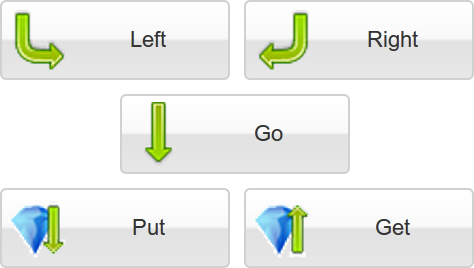
\includegraphics[width=6.2cm]{img/buttons-all-3.png}
\vspace{-6mm}
\end{center}
\end{figure}
\begin{enumerate}
\item[A1] North
\item[A2] South
\item[A3] East
\item[A4] West
\end{enumerate}  
\item Look at the button and decide which direction the robot is facing!
\begin{figure}[!ht]
\begin{center}
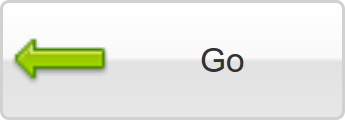
\includegraphics[width=3cm]{img/button-go-3.png}
\end{center}
\end{figure}
\begin{enumerate}
\item[A1] North
\item[A2] South
\item[A3] East
\item[A4] West
\end{enumerate}
\item Which direction is the robot facing after 
this button is pressed?
\begin{figure}[!ht]
\begin{center}

\includegraphics[width=3cm]{img/button-left-3.png}
\end{center}
\end{figure}
\begin{enumerate}
\item[A1] North
\item[A2] South
\item[A3] East
\item[A4] West
\end{enumerate}
\item What is the function of the following button?
\newpage

\begin{figure}[!ht]
\begin{center}

\includegraphics[width=3cm]{img/button-left-1.png}
\end{center}
\end{figure}
\begin{enumerate}
\item[A1] Make one step forward, turn left, and make one step forward.
\item[A2] Make one step forward and turn left
\item[A3] Step aside towards East and then make one step forward.
\item[A4] Turn left.
\end{enumerate}
\item The robot is facing North. Which button will make him face East?
\begin{enumerate}
\item[A1] 
\begin{figure}[!ht]
\begin{center}
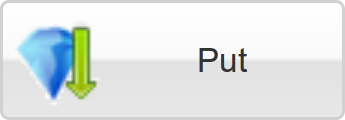
\includegraphics[width=3cm]{img/button-put-1.png}
\vspace{-10mm}
\end{center}
\end{figure}
\item[A2] 
\begin{figure}[!ht]
\begin{center}
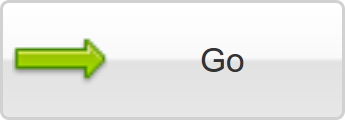
\includegraphics[width=3cm]{img/button-go-1.png}
\vspace{-10mm}
\end{center}
\end{figure}
\item[A3] 
\begin{figure}[!ht]
\begin{center}

\includegraphics[width=3cm]{img/button-right-2.png}
\vspace{-10mm}
\end{center}
\end{figure}
\item[A4] 
\begin{figure}[!ht]
\begin{center}

\includegraphics[width=3cm]{img/button-left-2.png}
\end{center}
\end{figure}
\end{enumerate}
\item The robot is facing South. Which two buttons do you need to press 
to make him move one step ahead and turn East?
\begin{enumerate}
\item[A1] 
\begin{figure}[!ht]
\begin{center}

\includegraphics[width=3cm]{img/button-go-4.png}\ \ \

\includegraphics[width=3cm]{img/button-left-4.png}
\end{center}
\end{figure}
\item[A2] 
\begin{figure}[!ht]
\begin{center}

\includegraphics[width=3cm]{img/button-go-4.png}\ \ \

\includegraphics[width=3cm]{img/button-right-4.png}
\end{center}
\end{figure}
\newpage
\item[A3] 
\begin{figure}[!ht]
\begin{center}
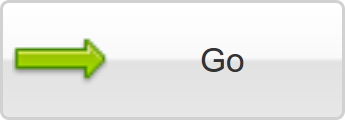
\includegraphics[width=3cm]{img/button-go-1.png}\ \ \

\includegraphics[width=3cm]{img/button-left-4.png}
\end{center}
\end{figure}
\item[A4] 
\begin{figure}[!ht]
\begin{center}
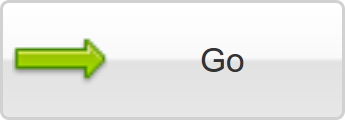
\includegraphics[width=3cm]{img/button-go-1.png}\ \ \

\includegraphics[width=3cm]{img/button-right-4.png}
\end{center}
\end{figure}
\end{enumerate}
\item Select one or more correct statements from the four options below!

\begin{figure}[!ht]
\begin{center}

\includegraphics[width=3cm]{img/button-left-1.png}\ \ \

\includegraphics[width=3cm]{img/button-left-2.png}\ \ \

\includegraphics[width=3cm]{img/button-left-3.png}\ \ \

\includegraphics[width=3cm]{img/button-left-4.png}
\end{center}
\end{figure}
\begin{enumerate}
\item[A1] All these buttons will turn the robot 90 degrees to the right.
\item[A2] Two of the buttons will turn the robot to the left, the other 
          two will turn him to the right.
\item[A3] The last button on the right will turn the robot to the left.
\item[A4] The last button on the right will turn the robot to the right.
\end{enumerate}

\item After you press the following button, the robot will:

\begin{figure}[!ht]
\begin{center}

\includegraphics[width=3cm]{img/button-right-4.png}
\end{center}
\end{figure}
\begin{enumerate}
\item[A1] Turn left and face West.
\item[A2] Turn right and face West.
\item[A3] Turn right and face East
\item[A4] Turn right and face South.
\end{enumerate}
\newpage
\item The robot is facing South. Which two buttons will make him rotate 180 degrees?

\begin{enumerate}
\item[A1] 
\begin{figure}[!ht]
\begin{center}

\includegraphics[width=3cm]{img/button-left-4.png}\ \ \

\includegraphics[width=3cm]{img/button-go-2.png}
\end{center}
\end{figure}
\item[A2] 
\begin{figure}[!ht]
\begin{center}

\includegraphics[width=3cm]{img/button-left-4.png}\ \ \

\includegraphics[width=3cm]{img/button-left-1.png}
\end{center}
\end{figure}
\item[A3] 
\begin{figure}[!ht]
\begin{center}

\includegraphics[width=3cm]{img/button-left-4.png}\ \ \

\includegraphics[width=3cm]{img/button-right-4.png}
\end{center}
\end{figure}
\item[A4] 
\begin{figure}[!ht]
\begin{center}
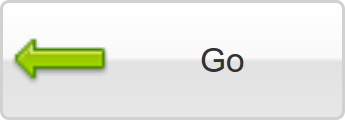
\includegraphics[width=3cm]{img/button-go-3.png}\ \ \

\includegraphics[width=3cm]{img/button-right-4.png}
\end{center}
\end{figure}
\end{enumerate}
\end{enumerate}

%%%%%%%%%%%%%%%%%%%%%%%%%%%%%%%%%%%%%%%%%%%%%%%%%%%%%%%%%%%%%%%%%%%%%%%%%%%%

\section{Programming Mode}

\begin{enumerate}
\item Where do we enter programs for Karel?
\begin{enumerate}
\item[A1] In Microsoft Word.
\item[A2] In Wordpad.
\item[A3] We upload them from hard disk.
\item[A4] In code cells.
\end{enumerate}
\item How are Karel's programs run?
\begin{enumerate}
\item[A1] By clicking on the green arrow in the menu.
\item[A2] By clicking on the green arrow under the code cell.
\item[A3] By clicking on Run in File menu.
\item[A4] By clicking on Run in Edit menu.
\end{enumerate}
\item The robot's initial situation is as shown in the image. His bag with gems is empty.
\begin{figure}[!ht]
\begin{center}
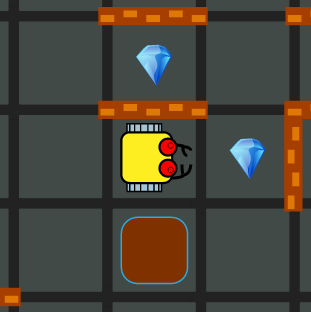
\includegraphics[width=4cm]{img/maze-0.png}
\end{center}
\end{figure}
\noindent
Read the following program and select one or more correct statements!
\begin{bluecode}
go
right
get
go
right 
go
\end{bluecode}
\begin{enumerate}
\item[A1] The robot will return home with no gems in the bag.
\item[A2] The robot will return home with one gem in the bag.
\item[A3] The robot will not return home and he will have no gems in the bag.
\item[A4] The robot will not return home and he will have one gem in the bag.
\end{enumerate}
\item The robot's initial situation is the same as in the previous question. He has no gems 
in his bag. Read the following program and select one or more correct statements from the four options below!
\begin{bluecode}
go
get
left
go
left
go
get
right
right
go
right
go
put
go
left 
go
\end{bluecode}
\begin{enumerate}
\item[A1] The robot will return home with two gems in the bag.
\item[A2] The robot will return home with only one gem in the bag.
\item[A3] The robot will not return home and he will have two gems in the bag.
\item[A4] The robot will not return home and he will have only one gem in the bag.
\end{enumerate}

\item What is an {\em algorithm}?
\begin{enumerate}
\item[A1] Very short program.
\item[A2] Sequence of instructions for the robot written using the correct commands.
\item[A3] Logical mistake in our program.
\item[A4] Sequence of logical steps written using human language.
\end{enumerate}
\item What is a {\em program}?
\begin{enumerate}
\item[A1] Sequence of logical steps written using human language.
\item[A2] Algorithm that does not contain any mistakes.
\item[A3] Algorithm that is translated from human language to programming language.
\item[A4] Very long algorithm.
\end{enumerate}
\item If the robot does something unexpected, what is the most probable reason for that?
\begin{enumerate}
\item[A1] Something is wrong with the computer.
\item[A2] Internet connection is too slow.
\item[A3] Web browser needs upgrading.
\item[A4] Our algorithm contains a logical mistake.
\end{enumerate}
\item What of the following is a {\em logical} mistake?
\begin{enumerate}
\item[A1] Mistake in an algorithm that causes the robot to do something unexpected.
\item[A2] Opening Karel through the Programming menu instead of through File Manager. 
\item[A3] Typing a command in a wrong way, such as {\tt lft} instead of {\tt left}.
\item[A4] Learning Fortran.
\end{enumerate}
\item What of the following is a {\em syntactical} mistake?
\begin{enumerate}
\item[A1] Writing {\tt left} instead of {\tt right}.
\item[A2] Having two empty characters between commands.
\item[A3] Mis-spelling a command.  
\item[A4] Mistake that causes the robot to do something unexpected.
\end{enumerate}
\item What of the following will cause an error message?
\begin{enumerate}
\item[A1] Turning the robot four times to the left.
\item[A2] Putting two or more gems on each other.
\item[A3] Using the {\tt put} command while the robot's bag is empty.
\item[A4] Returning home without any gems.
\end{enumerate}
\item What do we mean by {\em debugging}?
\begin{enumerate}
\item[A1] Apologizing after we ask a friend too many questions.
\item[A2] Playing an algorithm in our head prior to writing a program. 
\item[A3] Writing a new program after the previous one did not work.
\item[A4] Looking for mistakes in a program that does not work.
\end{enumerate}
\end{enumerate}

%%%%%%%%%%%%%%%%%%%%%%%%%%%%%%%%%%%%%%%%%%%%%%%%%%%%%%%%%%%%%%%%%%%%%%

\section{Counting Loop}

\begin{enumerate}
\item What command should we use to make the robot repeat something a given number of times?
\begin{enumerate}
\item[A1] {\tt repetition}
\item[A2] {\tt loop}
\item[A3] {\tt for}
\item[A4] {\tt repeat}
\end{enumerate}
\item Why should we always write one command per line?
\begin{enumerate}
\item[A1] To keep the code readable.
\item[A2] To make the code look longer.
\item[A3] Because all programming languages require that.
\item[A4] Because it speeds up communication with server.
\end{enumerate}
\item What is the {\em body} of a {\tt repeat} loop?
\begin{enumerate}
\item[A1] Body of a loop is the number that follows the {\tt repeat} command. 
\item[A2] The command on the first line following the {\tt repeat} command.
\item[A3] One or more commands that follow the {\tt repeat} command and are indented.
\item[A4] One or more commands that follow the {\tt repeat} command and are not indented.
\end{enumerate}
\item Why does the body of a loop need to be indented?
\begin{enumerate}
\item[A1] To make clear where it begins and where it ends.
\item[A2] It does not have to be indented, the indentation is optional.
\item[A3] Because the code is visually nicer.
\item[A4] Because the code is easier to read.
\end{enumerate}
\item Which program(s) will rotate Karel 360 degrees?
\begin{enumerate}
\item[A1] 
\begin{bluecode}
 left
 left
 left
 left
\end{bluecode}
\item[A2] 
\begin{bluecode}
 repeat 2
     right
     right
\end{bluecode}
\item[A3] 
\begin{bluecode}
 repeat 4
     left
\end{bluecode}
\item[A4] 
\begin{bluecode}
 repeat 2
     repeat 2
         right
\end{bluecode}
\end{enumerate}
\item Karel needs to pick up 5 gems from the ground, walk 10 steps forward, and put the 5 gems 
      on the ground again. Which one(s) of the following programs will do that?
\begin{enumerate}
\item[A1] 
\begin{bluecode}
 repeat 5
     get
     repeat 10
         go
         repeat 5
             put
\end{bluecode}
\item[A2] 
\begin{bluecode}
 repeat 5
     get
 repeat 10
     go
 repeat 5
     put
\end{bluecode}
\item[A3] 
\begin{bluecode}
 repeat 5
     get
     repeat 10
         go
     repeat 5
         put
\end{bluecode}
\item[A4] 
\begin{bluecode}
 repeat 5
 get
 repeat 10
 go
 repeat 5
 put
\end{bluecode}
\end{enumerate}
\end{enumerate}


\section{Working with Code and Text Cells}

\begin{enumerate}
\item How can a new text cell be added?
\begin{enumerate}
\item[A1] By clicking on {\em Add text cell} under an existing cell.
\item[A2] By clicking on {\em Add text cell} in the Edit menu.
\item[A3] By clicking on {\em New} in File menu.
\item[A4] By clicking on {\em Clone} in File menu.
\end{enumerate}
\item How can one add a new code cell?
\begin{enumerate}
\item[A1] Click on {\em Add new code cell} in the Edit menu.
\item[A2] Click on {\em New} in File menu.
\item[A3] Click on {\em Clone} in File menu.
\item[A4] Click on {\em Add code cell} under an existing cell.
\end{enumerate}
\item When should we use multiple code cells?
\begin{enumerate}
\item[A1] When our program contains more than one command.
\item[A2] When we want to run parts of the program separately.
\item[A3] When a command is repeated multiple times.
\item[A4] When the program is longer than 10 lines.
\end{enumerate}
\item What is the best way to erase all text from a cell?
\begin{enumerate}
\item[A1] Close Karel, logout, and login again. 
\item[A2] Restart Karel.
\item[A3] Remove the code cell and add a new one in its place.
\item[A4] Click on {\em Clear cell} under the cell.
\end{enumerate}
\item How can a cell be collapsed?
\begin{enumerate}
\item[A1] Click on {\em Remove cell} under the cell.
\item[A2] Click on {\em Collapse cell} under the cell.
\item[A3] Click on {\em Collapse} in File menu.
\item[A4] Click on the bracket on the right of the cell.
\end{enumerate}
\item How can a cell be removed?
\begin{enumerate}
\item[A1] Click on {\em Add code cell} under the cell.
\item[A2] Click on {\em Remove cell} under the cell.
\item[A3] Click on {\em Clear cell} under the cell.
\item[A4] Switch to Designer and back.
\end{enumerate}
\item How can we evaluate all code cells at once?
\begin{enumerate}
\item[A1] Through {\em Expand all cells} in Edit menu.
\item[A2] Click on the red button in the main menu.
\item[A3] Click on {\em Run cell} under the last code cell.
\item[A4] Click on the green arrow button in the main menu.
\end{enumerate}
\item How should a running program be stopped?
\begin{enumerate}
\item[A1] Click on the green arrow button in the main menu.
\item[A2] Close the main Karel window.
\item[A3] Click on the red button in the main menu.
\item[A4] Click on {\em stop} under the last code cell.
\end{enumerate}
\item How can we evaluate just one selected code cell?
\begin{enumerate}
\item[A1] Copy and paste the contents of all 
          code cells into the first one, and remove them.
\item[A2] Click on the green arrow button in the main menu. 
\item[A3] Click on the green arrow button under the code cell.
\item[A4] Click on {\em Remove cell} under the code cell.
\end{enumerate}
\end{enumerate}

%%%%%%%%%%%%%%%%%%%%%%%%%%%%%%%%%%%%%%%%%%%%%%%%%%%%%%%%%%%%%%%%%%%%%%

\section{Conditions}

\begin{enumerate}
\item When does the {\tt gem} sensor check true?
\begin{enumerate}
\item[A1] There is at least one gem in the maze.
\item[A2] There is at least one gem in front of the robot.
\item[A3] There are one or more gems under the robot.
\item[A4] The robot's bag contains at least one gem.
\end{enumerate}
\item When does the {\tt north} sensor check true?
\begin{enumerate}
\item[A1] The robot's home is North of him.
\item[A2] The robot is North of his home.
\item[A3] The robot faces South.
\item[A4] The robot faces North.
\end{enumerate}
\item When does the {\tt empty} sensor check true?
\begin{enumerate}
\item[A1] The robot's bag is empty.
\item[A2] There are no gems where the robot stands.
\item[A3] There are no gems in the maze.
\item[A4] There are no gems in the robot's home.
\end{enumerate}
\item When does the {\tt home} sensor check true?
\begin{enumerate}
\item[A1] Robot's home is right in front of the robot.
\item[A2] The robot is inside his home.
\item[A3] Robot's home is straight ahead of the robot.
\item[A4] The robot needs to go home to drop all gems that he collected.
\end{enumerate}
\item When does the {\tt wall} sensor check true?
\begin{enumerate}
\item[A1] The robot will reach a wall with one or more steps. 
\item[A2] There is a wall on the robot's right-hand side.
\item[A3] There is a wall right in front of the robot.
\item[A4] There is a wall on the robot's left-hand side.
\end{enumerate}
\item When can Karel see from where he stands whether a wall is two steps ahead?
\begin{enumerate}
\item[A1] Never.
\item[A2] If his home is not in the way.
\item[A3] If no gem is in the way.
\item[A4] If no other wall is in the way.
\end{enumerate}
\item When can the robot check without turning whether a wall is on his right?
\begin{enumerate}
\item[A1] Any time, there is the sensor {\tt right} for that.
\item[A2] Any time, there is the sensor {\tt wall} for that.
\item[A3] Only if he is not at home.
\item[A4] Never.
\end{enumerate}
\item Can Karel check from where he stands whether a gem is one step away?
\begin{enumerate}
\item[A1] Yes, there is the sensor {\tt gem} for that.
\item[A2] No.
\item[A3] Yes but the gem must be in front of him.
\item[A4] Yes but not when he is at home.
\end{enumerate}
\item Can he check from where he stands whether his home is one step away?
\begin{enumerate}
\item[A1] Yes but his home must be in front of him.
\item[A2] Yes, there is the sensor {\tt home} for that.
\item[A3] No.
\item[A4] Yes but not when he is at home.
\end{enumerate}
\item Can the robot check whether he has at least one gem in the bag?
\begin{enumerate}
\item[A1] No.
\item[A2] Yes, he can use the {\tt gem} sensor. 
\item[A3] No, the sensor gem only works for one gem.
\item[A4] Yes, he can use the {\tt empty} sensor.
\end{enumerate}
\item Which program(s) make Karel check whether he stands on a gem, and if so, to pick it up?
\begin{enumerate}
\item[A1] 
\begin{bluecode}
if gem
    get
\end{bluecode}
\item[A2] 
\begin{bluecode}
if not empty
    get
\end{bluecode}
\item[A3] 
\begin{bluecode}
if get
    gem
\end{bluecode}
\item[A4] 
\begin{bluecode}
if empty
    get
\end{bluecode}
\end{enumerate}
\item Which program(s) will turn Karel to the North, regardless the direction he is facing?
\begin{enumerate}
\item[A1] 
\begin{bluecode}
repeat 4
    if not north 
        left
\end{bluecode}
\item[A2] 
\begin{bluecode}
if not north 
    left
else 
    right
\end{bluecode}
\item[A3] 
\begin{bluecode}
if south
    repeat 2
        right
\end{bluecode}
\item[A4] 
\begin{bluecode}
if not north 
    right
\end{bluecode}
\end{enumerate}
\end{enumerate}


%%%%%%%%%%%%%%%%%%%%%%%%%%%%%%%%%%%%%%%%%%%%%%%%%%%%%%%%%%%%%%%%%%%%%%

\section{Conditional Loop}

\begin{enumerate}
\item What is the difference between the {\tt repeat} and {\tt while} loops?
\begin{enumerate}
\item[A1] Body of the {\tt while} loop does not have to be indented.
\item[A2] The {\tt while} loop only can be used when the number of repetitions is known a priori.
\item[A3] The {\tt repeat} loop can do 100 repetitions maximum.
\item[A4] The {\tt repeat} loop only can be used when the number of repetitions is known a priori.
\end{enumerate}
\item Which program will always turn Karel to face West?
\begin{enumerate}
\item[A1] 
\begin{bluecode}
repeat 4
    left
\end{bluecode}
\item[A2] 
\begin{bluecode}
while not west
    right
\end{bluecode}
\item[A3] 
\begin{bluecode}
while not north
    left
left
\end{bluecode}
\item[A4] 
\begin{bluecode}
while not north 
    right
left
\end{bluecode}
\end{enumerate}
\item The maze does not contain any gems and any walls except for the ones that 
      form the outer rectangular boundary.
      The robot stands in the south-west corner facing East. Which program will 
      make the robot walk along the 
      boundary of the maze and bring him back to the original position?
\begin{enumerate}
\item[A1] 
\begin{bluecode}
repeat 4
    while not wall
        go
\end{bluecode}
\item[A2] 
\begin{bluecode}
repeat 4
    while not wall
        go
    left
\end{bluecode}
\item[A3] 
\begin{bluecode}
repeat 4
    while not wall
        go
    right
\end{bluecode}
\item[A4] 
\begin{bluecode}
repeat 4
    while not wall
        left
    go
\end{bluecode}
\end{enumerate}
\end{enumerate}

%%%%%%%%%%%%%%%%%%%%%%%%%%%%%%%%%%%%%%%%%%%%%%%%%%%%%%%%%%%%%%%%%%%%%%

\section{Custom Commands}

\begin{enumerate}
\item Should we, or should we not always try to split a big task into smaller ones?
\begin{enumerate}
\item[A1] No, because it makes the resulting program longer.
\item[A2] Yes, because then we can only solve the simple tasks.
\item[A3] Yes, because then we can ask help solving some tasks.
\item[A4] Yes, because the big task becomes simpler to solve.
\end{enumerate}
\item Should we, or should we not replicate computer code?
\begin{enumerate}
\item[A1] Yes, because the resulting program is faster.
\item[A2] Yes, because the resulting program is simpler.
\item[A3] No, because our code would become prone to errors.
\item[A4] No, because the Karel language does not allow that.
\end{enumerate}
\item When should a new command be defined?
\begin{enumerate}
\item[A1] Whenever the same command is repeated on two consecutive lines in the code.
\item[A2] Whenever the algorithm contains an action that is repeated in
          more than one situation.
\item[A3] Whenever the code contains an {\tt if - else} statement.
\item[A4] If the code is longer than 100 lines.
\end{enumerate}
\item Which command(s) will empty the robot's bag without causing an error?
\begin{enumerate}
\item[A1] 
\begin{bluecode}
def emptybag
    while gem
        put
\end{bluecode}
\item[A2] 
\begin{bluecode}
def emptybag
    while not gem
        put
\end{bluecode}
\item[A3] 
\begin{bluecode}
def emptybag
    while empty
        put
\end{bluecode}
\item[A4] 
\begin{bluecode}
def emptybag
    while not empty
        put
\end{bluecode}
\end{enumerate}
\item Which command(s) will turn Karel to the South no matter 
      which direction he is facing?
\begin{enumerate}
\item[A1] 
\begin{bluecode}
def turnsouth
    while north
        repeat 2
            left
\end{bluecode}
\item[A2] 
\begin{bluecode}
def turnsouth
    while not north
        right
    repeat 2
        left
\end{bluecode}
\item[A3] 
\begin{bluecode}
def turnsouth
    while not north
        right
    repeat 2
        right
\end{bluecode}
\item[A4] 
\begin{bluecode}
def turnsouth
    while not north
        left
    repeat 2
        left
\end{bluecode}
\end{enumerate}
\end{enumerate}


%%%%%%%%%%%%%%%%%%%%%%%%%%%%%%%%%%%%%%%%%%%%%%%%%%%%%%%%%%%%%%%%%%%%%%

\section{Recursion}

\begin{enumerate}
\item There are three commands {\tt A}, {\tt B}, {\tt C}. Identify all cases of recursion in the four options below!
\begin{enumerate}
\item[A1] {\tt C} calls {\tt B}, {\tt B} calls {\tt A}, {\tt C} calls {\tt A}.
\item[A2] {\tt C} calls {\tt B}, {\tt B} calls {\tt C}, {\tt C} calls {\tt A}.
\item[A3] {\tt C} calls {\tt B}, {\tt B} calls {\tt A}, {\tt A} calls {\tt C}.
\item[A4] {\tt C} calls {\tt B}, {\tt B} calls {\tt A}, {\tt A} calls {\tt B}.
\end{enumerate}
\item What do we mean by {\em base case} in recursion?
\begin{enumerate}
\item[A1] The initial state of the robot before executing a recursive program.
\item[A2] Recursion where a single command calls itself directly.
\item[A3] Branch of a conditional statement that makes a recursive call.
\item[A4] Branch of a conditional statement that does not make a recursive call.
\end{enumerate}
\item What happens if base case is not present?
\begin{enumerate}
\item[A1] Recursion turns into an infinite loop.
\item[A2] The program throws an error.
\item[A3] The program will end after the first call to the recursive command.
\item[A4] The program does not throw an error but the robot will do nothing.
\end{enumerate}
\item When should recursion be used?
\begin{enumerate}
\item[A1] The algorithm contains multiple conditional statements.
\item[A2] The algorithm contains multiple repetitions.
\item[A3] After solving part of the problem, the remaining task is similar to the original problem.
\item[A4] Our program contains multiple new commands.
\end{enumerate}
\item Which of the four recursive commands below 
turn(s) the robot to the North without causing an infinite loop?
\begin{enumerate}
\item[A1]
\begin{bluecode}
def turn_north
    right
    turn_north
\end{bluecode}
\item[A2] 
\begin{bluecode}
def turn_north
    if not north
        right
    turn_north
\end{bluecode}
\item[A3] 
\begin{bluecode}
def turn_north
    if not north
        right
        turn_north
\end{bluecode}
\item[A4] 
\begin{bluecode}
def turn_north
    right
    if not north 
        turn_north
\end{bluecode}
\end{enumerate}
\end{enumerate}

%%%%%%%%%%%%%%%%%%%%%%%%%%%%%%%%%%%%%%%%%%%%%%%%%%%%%%%%%%%%%%%%%%%%%%

\section{Variables and Functions}

\begin{enumerate}
\item What are {\em variables} used for in programming? 
\begin{enumerate}
\item[A1] To generate random data.
\item[A2] To make programs shorter.
\item[A3] To store useful information.
\item[A4] To create variable mazes.
\end{enumerate}
\item What values do the read-only variables {\tt gpsx} and {\tt gpsy} have when Karel's
position is as shown in Fig. \ref{fig:var2}?

\begin{figure}[!ht]
\begin{center}
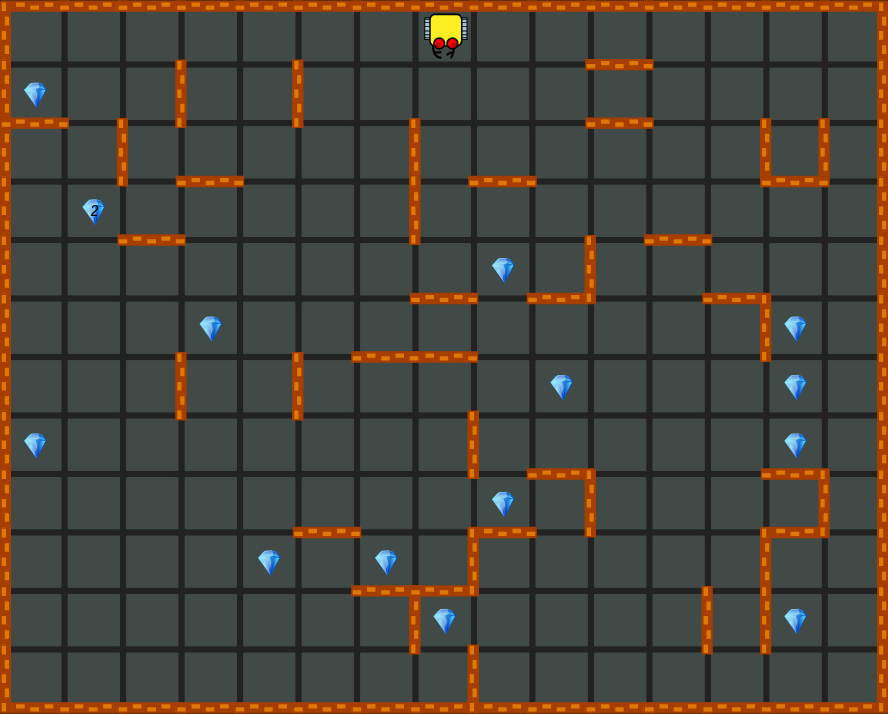
\includegraphics[height=0.4\textwidth]{img/variables2.png}
\end{center}
\vspace{-4mm}
\caption{Karel is reading his GPS device again.}
\label{fig:var2}
%\vspace{-1cm}
\end{figure}
\noindent

\begin{enumerate}
\item[A1] {\tt gpsx} is 7 and {\tt gpsy} is 12.
\item[A2] {\tt gpsx} is 8 and {\tt gpsy} is 0.
\item[A3] {\tt gpsx} is 8 and {\tt gpsy} is 12.
\item[A4] {\tt gpsx} is 7 and {\tt gpsy} is 11.
\end{enumerate}
\item What values will the variables {\tt gpsx} and {\tt gpsy} have after
Karel executes the following program? He starts from the position shown 
in Fig. \ref{fig:var2}.
\begin{bluecode}
repeat 5
    while not wall
        go
        if gem
            get
    left
\end{bluecode}
\begin{enumerate}
\item[A1] {\tt gpsx} is 7 and {\tt gpsy} is 7.
\item[A2] {\tt gpsx} is 0 and {\tt gpsy} is 10.
\item[A3] {\tt gpsx} is 9 and {\tt gpsy} is 7.
\item[A4] {\tt gpsx} is 9 and {\tt gpsy} is 11.
\end{enumerate}
\item Which of the following programs are invalid?
\begin{enumerate}
\item[A1] 
\begin{bluecode}
a = gpsx
inc(a)
\end{bluecode}
\item[A2] 
\begin{bluecode}
b = 7
dec(b)
\end{bluecode}
\item[A3] 
\begin{bluecode}
gpsx = 0
inc(gpsx)
\end{bluecode}
\item[A4] 
\begin{bluecode}
e = 1
e = gpsx
e = gpsy
\end{bluecode}
\end{enumerate}
\item Which of the following programs are invalid?
\begin{enumerate}
\item[A1] 
\begin{bluecode}
def count_steps
    n = 0
    while not wall
        go
        inc(n)
    return n
\end{bluecode}
\item[A2] 
\begin{bluecode}
def count_steps
    n = 0
    while not wall
        go
        inc(n, 1)
    print "Number of steps made =", n
\end{bluecode}
\item[A3] 
\begin{bluecode}
def count_steps
    n = 0
    while not wall
        go
        inc(n)
\end{bluecode}
\item[A4] 
\begin{bluecode}
def count_steps
    while not wall
        go
        inc(n)
    return n
\end{bluecode}
\end{enumerate}
\end{enumerate}

%%%%%%%%%%%%%%%%%%%%%%%%%%%%%%%%%%%%%%%%%%%%%%%%%%%%%%%%%%%%%%%%%%%%%%

\section{Lists}

\begin{enumerate}
\item Which of the following are correct ways to define a list?
\begin{enumerate}
\item[A1] 
\begin{bluecode}
L = []
\end{bluecode}
\item[A2] 
\begin{bluecode}
L = [1, 2, 35]
\end{bluecode}
\item[A3] 
\begin{bluecode}
L = [20, "Monday", [5, 15]]
\end{bluecode}
\item[A4] 
\begin{bluecode}
word = "Monday"
list = [5, 15]
L = [20, word, list]
\end{bluecode}
\end{enumerate}
\item What is the correct way to store the length of list {\tt L}
in variable {\tt m}?
\begin{enumerate}
\item[A1] 
\begin{bluecode}
m = L
\end{bluecode}
\item[A2] 
\begin{bluecode}
m = length(L)
\end{bluecode}
\item[A3] 
\begin{bluecode}
m = len(L)
\end{bluecode}
\item[A4] 
\begin{bluecode}
m = L[0]
\end{bluecode}
\end{enumerate}
\item List {\tt Y} is defined as {\tt [1, 4, 9]}. Which of the 
following codes will throw an error?
\begin{enumerate}
\item[A1] 
\begin{bluecode}
print Y[0]
\end{bluecode}
\item[A2] 
\begin{bluecode}
a = L[1]
\end{bluecode}
\item[A3] 
\begin{bluecode}
b = L[2]
\end{bluecode}
\item[A4] 
\begin{bluecode}
print L[3]
\end{bluecode}
\end{enumerate}
\item Which of the following are correct ways to append {\tt 100} to a list {\tt X}?
\begin{enumerate}
\item[A1] 
\begin{bluecode}
append(X, 100)
\end{bluecode}
\item[A2] 
\begin{bluecode}
X.append(100)
\end{bluecode}
\item[A3] 
\begin{bluecode}
append(100, X))
\end{bluecode}
\item[A4] 
\begin{bluecode}
100.append(X)
\end{bluecode}
\end{enumerate}
\item List {\tt Z} is defined as {\tt ["January", "February", "March"]}.
Which of the following codes will remove the last item from {\tt Z} 
and assign it to the variable {\tt month}?
\begin{enumerate}
\item[A1] 
\begin{bluecode}
month = Z.pop()
\end{bluecode}
\item[A2] 
\begin{bluecode}
month = Z[2]
\end{bluecode}
\item[A3] 
\begin{bluecode}
month = del Z[2]
\end{bluecode}
\item[A4] 
\begin{bluecode}
month = Z.pop(2)
\end{bluecode}
\end{enumerate}
\end{enumerate}

%%%%%%%%%%%%%%%%%%%%%%%%%%%%%%%%%%%%%%%%%%%%%%%%%%%%%%%%%%%%%%%%%%%%%%

\section{Logic}

\begin{enumerate}
\item Let's introduce a variable {\tt my\_age} that stores your age in years.
      This variable is:
\begin{enumerate}
\item[A1] Numerical.
\item[A2] Logical.
\item[A3] Both numerical and logical.
\item[A4] Neither numerical nor logical.
\end{enumerate}
\item What is a {\em logical expression}? 
\begin{enumerate}
\item[A1] Expression that makes sense.
\item[A2] Expression that is always true. 
\item[A3] Expression that is either true or false.
\item[A4] Expression that cannot be false.
\end{enumerate}
\item A is {\tt True} and B is {\tt False}. What is then the value of (A {\em and} B) ?
\begin{enumerate}
\item[A1] {\tt False}.
\item[A2] {\tt True}.
\item[A3] It can be both {\tt True} and {\tt False}.
\item[A4] Neither {\tt True} nor {\tt False}.
\end{enumerate}
\item A is {\tt True} and B is {\tt False}. What is then the value of (A {\em or} B) ?
\begin{enumerate}
\item[A1] {\tt False}.
\item[A2] {\tt True}.
\item[A3] It can be both {\tt True} and {\tt False}.
\item[A4] Neither {\tt True} nor {\tt False}.
\end{enumerate}
\item A is {\tt True} and B is {\tt False}. What is then the value of (A {\em and} {\em not} (A {\em or} B)) ?
\begin{enumerate}
\item[A1] {\tt False}.
\item[A2] {\tt True}.
\item[A3] It can be both {\tt True} and {\tt False}.
\item[A4] Neither {\tt True} nor {\tt False}.
\end{enumerate}
\item A is {\tt True} and B is {\tt True}. What is then the value of (A {\em and} {\em not} (A {\em and} {\em not} B)) ?
\begin{enumerate}
\item[A1] {\tt False}.
\item[A2] {\tt True}.
\item[A3] It can be both {\tt True} and {\tt False}.
\item[A4] Neither {\tt True} nor {\tt False}.
\end{enumerate}
\end{enumerate}

%%%%%%%%%%%%%%%%%%%%%%%%%%%%%%%%%%%%%%%%%%%%%%%%%%%%%%%%%%%%%%%%%%%%%%%%%%%%%%%%%%%%%%%%


%%%%%%%%%%%%%%%%%%%%%%%%%%%%%%%%%%%%%%%%%%%%%%%%%%%%%%%%%%%%%%%%%%%%%

